% Sets page margins to 1", which is the academic standard
% allows the included extensions of graphic files
% sets graphic path, does not currently work because of space in folder name
% I do not remember what this does
% allows the xhead parameters (text on the top right/left areas of pages)
% \setcounter{tocdepth}{the number of depth}
% INCLUDEGRAPHICS EXPLANATION
% \includegraphics[scale=1]{name of file}
% sometimes you want to twice encase the filename in squiggly brackets. I do not know why but sometimes it is required.


\documentclass{article}
%%%%%%%%%%%%%%%%%%%%%%%%%%%%%%%%%%%%%%%%%%%%%%%%%%%%%%%%%%%%%%%%%%%%%%%%%%%%%%%%%%%%%%%%%%%%%%%%%%%%%%%%%%%%%%%%%%%%%%%%%%%%%%%%%%%%%%%%%%%%%%%%%%%%%%%%%%%%%%%%%%%%%%%%%%%%%%%%%%%%%%%%%%%%%%%%%%%%%%%%%%%%%%%%%%%%%%%%%%%%%%%%%%%%%%%%%%%%%%%%%%%%%%%%%%%%
\usepackage{geometry}
\usepackage{fancyhdr}
\usepackage[pdftex]{graphicx}

%TCIDATA{OutputFilter=LATEX.DLL}
%TCIDATA{Version=5.50.0.2953}
%TCIDATA{<META NAME="SaveForMode" CONTENT="1">}
%TCIDATA{BibliographyScheme=Manual}
%TCIDATA{Created=Monday, January 30, 2012 17:20:46}
%TCIDATA{LastRevised=Monday, March 12, 2012 12:19:36}
%TCIDATA{<META NAME="GraphicsSave" CONTENT="32">}
%TCIDATA{<META NAME="DocumentShell" CONTENT="Standard LaTeX\Blank - Standard LaTeX Article">}
%TCIDATA{CSTFile=40 LaTeX article.cst}

\newtheorem{theorem}{Theorem}
\newtheorem{acknowledgement}[theorem]{Acknowledgement}
\newtheorem{algorithm}[theorem]{Algorithm}
\newtheorem{axiom}[theorem]{Axiom}
\newtheorem{case}[theorem]{Case}
\newtheorem{claim}[theorem]{Claim}
\newtheorem{conclusion}[theorem]{Conclusion}
\newtheorem{condition}[theorem]{Condition}
\newtheorem{conjecture}[theorem]{Conjecture}
\newtheorem{corollary}[theorem]{Corollary}
\newtheorem{criterion}[theorem]{Criterion}
\newtheorem{definition}[theorem]{Definition}
\newtheorem{example}[theorem]{Example}
\newtheorem{exercise}[theorem]{Exercise}
\newtheorem{lemma}[theorem]{Lemma}
\newtheorem{notation}[theorem]{Notation}
\newtheorem{problem}[theorem]{Problem}
\newtheorem{proposition}[theorem]{Proposition}
\newtheorem{remark}[theorem]{Remark}
\newtheorem{solution}[theorem]{Solution}
\newtheorem{summary}[theorem]{Summary}
\newenvironment{proof}[1][Proof]{\noindent\textbf{#1.} }{\ \rule{0.5em}{0.5em}}
\geometry{left=1in,right=1in,top=1in,bottom=1in} 
\DeclareGraphicsExtensions{.pdf,.png,.jpg}
\graphicspath{{D:/Dropbox/Private/FP/Gruppe34/FellesDoc/Ktn/}}
\setlength{\headheight}{15.2pt}
\pagestyle{fancy}
\lhead{Gruppe 34}
\rhead{FP: KTN1 Phase 1}
\input{tcilatex}
\setcounter{secnumdepth}{1}

\begin{document}


% begin title page, use \\ for newline
\begin{titlepage}
\title{Collaboration Project\\
\textbf{KTN1 Phase 1}\\
Gruppe 34}
% now one can list the authors, \textbf{} makes bold text
\author{Bj\o rn \AA ge Tungesvik\and Tina Syversen\and Andr\'e Philipp\and Odd Magnus Trondrud\and Eivind Kvissel\and H\aa vard H\o iby}
\maketitle
\end{titlepage}\qquad 

\part{The Design}

\section{Connection}

TCP employs a three way handshake to create a connection between two hosts.
This functionality can be realized by implementing the \texttt{connect()}
and \texttt{accept()} methods mentioned in the connection interface. The 
\texttt{connect()} method will handle the client side of the handshake,
while \texttt{accept()} will handle the server side.

\bigskip

The TCP client starts in the closed state. A new TCP is initiated by sending
a packet with the \texttt{SYN} bit set to 1, and its randomly chosen
internal sequence number. After the \texttt{SYN} segement is sent, the
client enters the \texttt{\texttt{SYN}\_SENT} state, waiting for the
corresponding \texttt{\texttt{SYN}\_ACK} from the server.

\bigskip

The server will respond to the \texttt{SYN} packet by sending a \texttt{%
\texttt{SYN}\_ACK} packet, with the \texttt{SYN} bit set to 1, its internal
sequence number, and the \texttt{ACK} field set to the next expected
sequence number.

\bigskip

When the client has received the \texttt{\texttt{SYN}\_ACK} packet, it
enters the \texttt{ESTABLISHED} state, and sends an \texttt{ACK} packet,
informing the server that the \texttt{\texttt{SYN}\_ACK} packet was
received. When the server receives the \texttt{ACK} packet, the server
enters the \texttt{ESTABLISHED} state.

\subsection{connect()}
\includegraphics[scale=0.95]{ktnConnect.pdf}
\subsection{accept()}
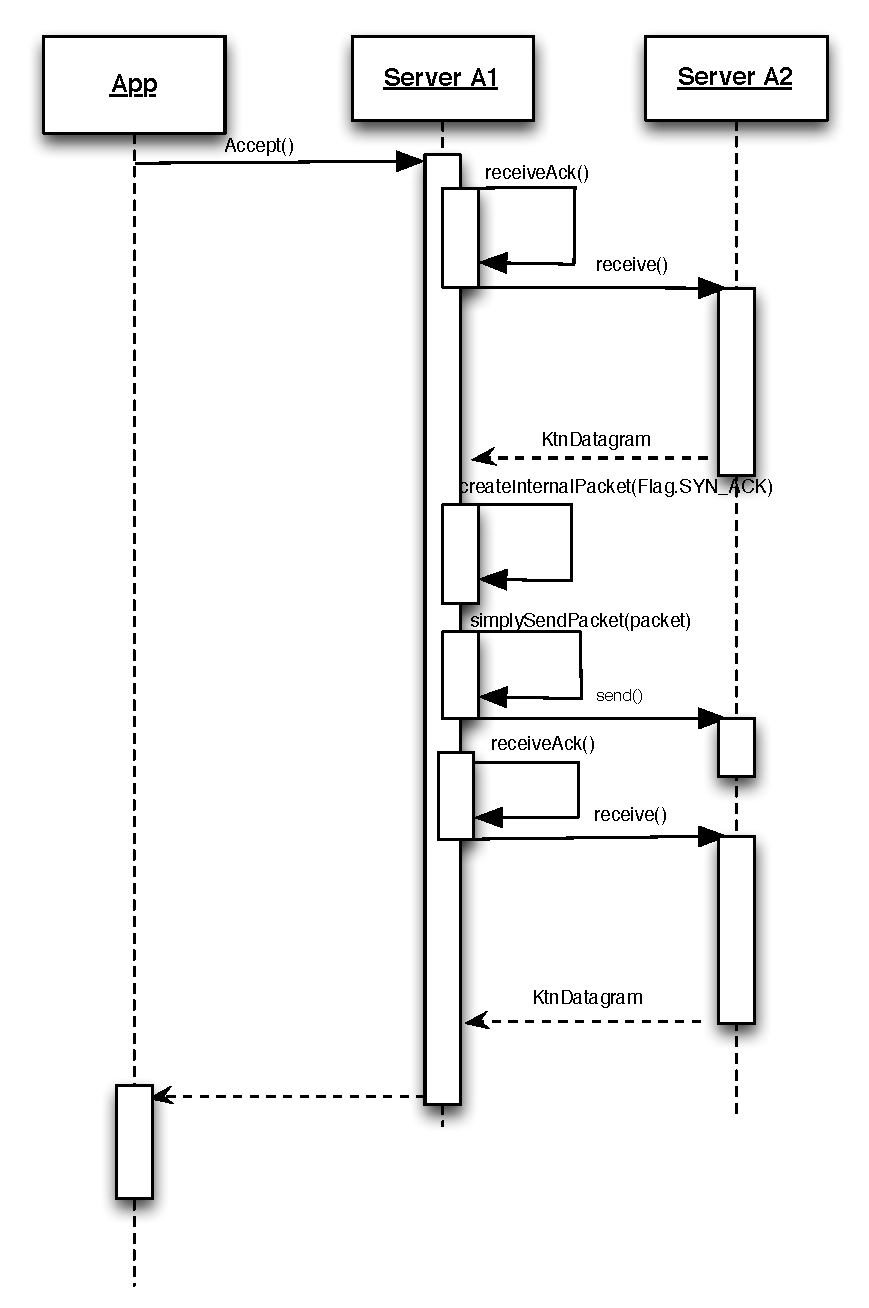
\includegraphics[scale=0.95]{ktnAccept.pdf}
\subsection{receive()}
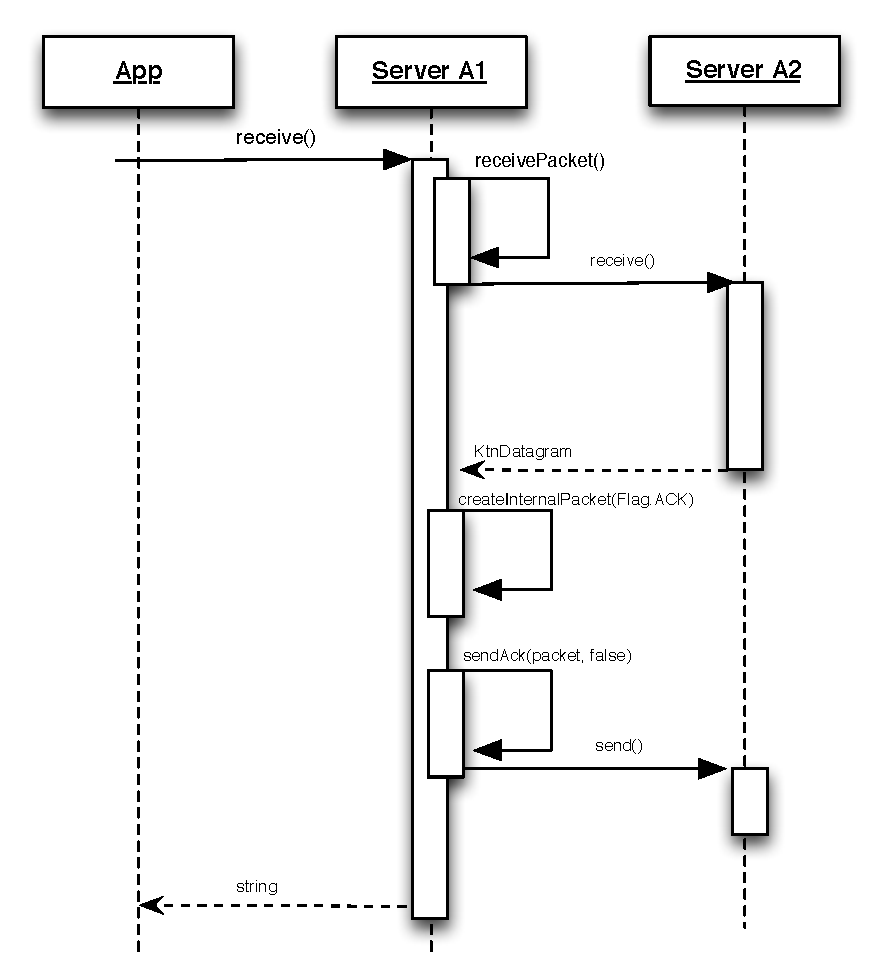
\includegraphics[scale=0.95]{ktnRecv.pdf}
\subsection{send()}
\includegraphics[scale=0.95]{ktnSend.pdf}
\newpage
\section{Disconnection}

For this discussion, lets presume that the clients initiate the close
operation using the \texttt{close()} method (Note: the server can also use the close
operation). This causes the client to send a \texttt{SYN} packet with the 
\texttt{FIN} bit set to 1, and enter the \texttt{FIN\_WAIT\_1}.
While in the \texttt{FIN\_WAIT\_1} state the client waits for an 
\texttt{ACK} packet. Upon receiving the \texttt{ACK} packet the client
switches to \texttt{FIN\_WAIT\_2} state.

\bigskip

In \texttt{FIN\_WAIT\_2} state the client is expecting a \texttt{FIN%
} packet from the server. As mentioned above, it's possible to receive the 
\texttt{FIN} packet directly. Anyway, when the \texttt{FIN} packet is
received, the client will respond with an \texttt{ACK} packet, and enter the
\texttt{\texttt{TIME\_WAIT}} state. This state allows the client to re-send the last final 
\texttt{ACK} packet in case its lost. After the waiting period, the client
formally closes the connection.

\bigskip

The server will receive the \texttt{FIN} packet, send an \texttt{ACK} packet
as a response, and enter the \texttt{CLOSE\_WAIT} state. While in the close wait
state, the server sends a \texttt{FIN} packet to the client, and enters the 
\texttt{LAST\_ACK} state. In this state the server wait for a \texttt{ACK}
packet from the client. When the packet is finally received, the connection
is finally closed.

\bigskip

Note: The server can also terminate a connection, thereby switching roles
with the client.

\subsection{\texttt{close()}}
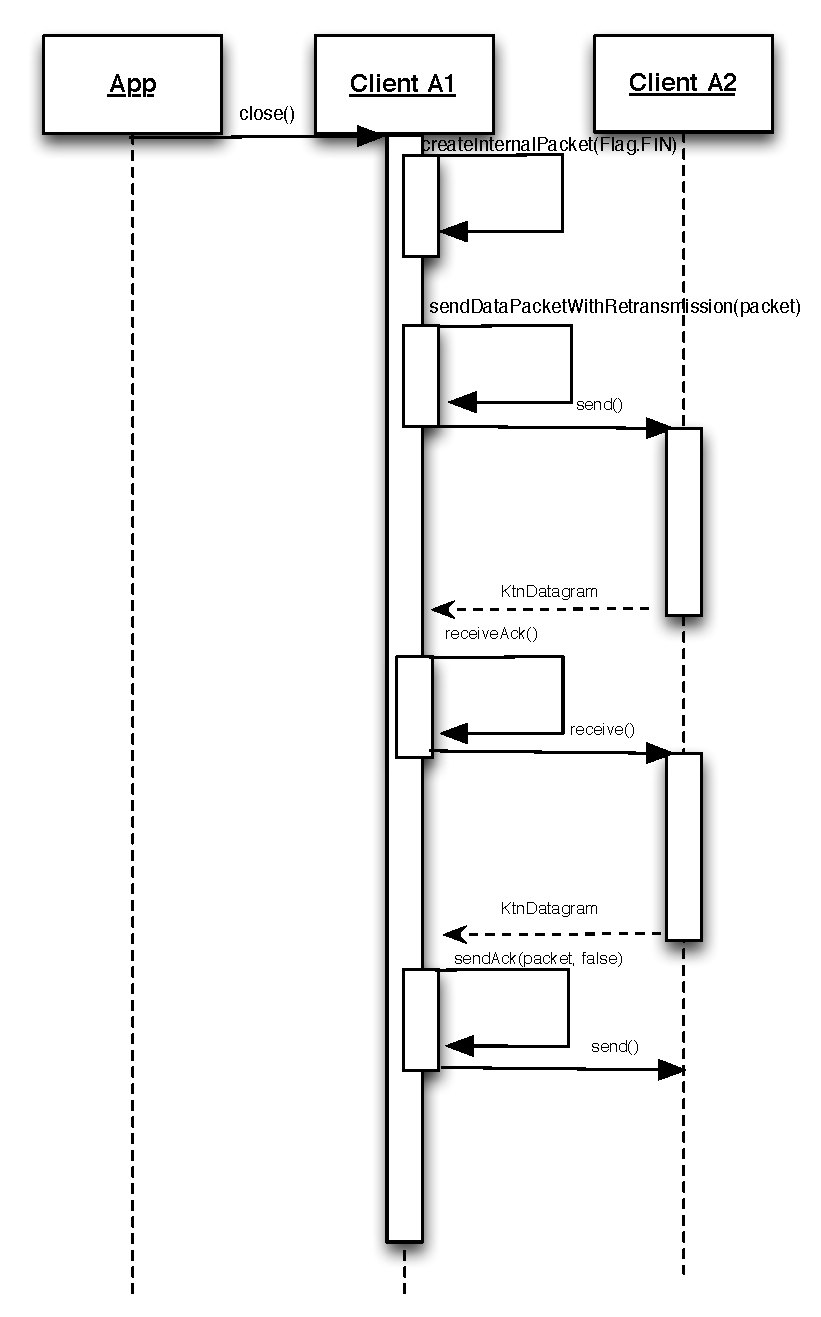
\includegraphics[scale=0.95]{ktnClientClose.pdf}
\subsection{ServerClose}
\includegraphics[scale=0.95]{ktnServerClose.pdf}

\subsection{ServerClose}

\section{Error Handling}

\subsection{Packet Loss}

When sending a packet the receiver of the packet will ask about it until the
packet is received. The packet is timed so that if the sender does not
receive an \texttt{ACK} during a given time(timeout), the sender will send
the packet again.

\subsection{Packet Delay}

A1 saves all the packets in a buffer, but it does not store duplicates. So
when the sender does not receive an \texttt{ACK}, it believes that the
packet is lost and sends it again. This means that the receiver gets two of
the same packet. This problem can be solved by checking the sequence number.
If a packet with the same sequence number has already been received, the
packet will be dropped, but the receiver will still send an \texttt{ACK} for
the duplicated packet.

\subsection{Packet Error/Corruption}

Right before a message is received it will be checked for errors using a
checksum to see if the packet contains any errors. If the packet does
contain errors an \texttt{ACK} will be sent, saying that the packet contains
errors.

\subsection{Ghost Packets}

The checksum will be checked and if it does not chek out be discarded. If it
is approved, the sequence number will be checked. If it does not have the
right sequence number it will be thrown away, if not it will be approved as
an ordinary packet.

\subsection{Packet Checks Out}

If the packet checks out it will be passed on upwards.

\newpage
\part{The Tests}

\section{Testing Plan}

The tests in this plan are laid out in an incremental fashion. First tests
will be performed for all features (connection, tear down, send and receive)
without errors enabled to ensure that everything works in a trivial
environment. Then each error will be added one by one. After two errors have
been tested individually those two are tested in combination, when three
errors have been tested all three errors will be tested together. And so on
until all errors are accounted for.

\subsection{Error Probability}

Each test case, containing errors, will be run twice at 10\% and 50\% error
rate in conjunction with the specifications (ref: Kompendium for
Fellesprosjektet chap. 6.3.1).

\subsection{Test repetition}

All test containing the sending and reception of an actual payload will
dispatch 10 distinct payloads, in order to evaluate the received payloads
precisely.

\section{Initial Connection (no errors enabled)\ - T-KTN01}

\subsection{Preconditions}

Methods \texttt{connect()} and \texttt{accept()} must be implemented in A1 (%
\texttt{ConnectionImpl}). The \texttt{errors} variable in \texttt{%
settings.xml} should be false.

\subsection{Dependencies}

NA

\subsection{Objective}

Setup a connection between two hosts running the same implementation of A1. 

\subsection{Instructions}

This is done by creating a \texttt{ConnectionImpl} object on both the server
and the client side. First the server executes the \texttt{accept()} method
with port X, then the client executes the method \texttt{connect()} with the
server IP and port X.

\subsection{Expected Result}

A three-way handshake should be observed. This can be verified on the client
side by the \texttt{connect()} method returning without throwing a \texttt{%
SocketTimeoutException}. On the server side the test is passed if the accept
method returns a \texttt{Connection} as opposed to throwing a \texttt{%
SocketTimeoutException}.

\section{Connection and Tear Down}

\subsection{Preconditions}

The \texttt{close()} method must be implemented in A1 (\texttt{ConnectionImpl%
}). The \texttt{errors} variable in \texttt{settings.xml} should be false.

\subsection{Dependencies}

\textbf{T-KTN01}

\subsection{Objective}

Close a connection between two hosts running the same implementation of A1.

\subsection{Instructions}

This is done by first creating a connection as described in \textbf{T-KTN01}%
. After the connection is established either the client or the server calls
the \texttt{close()}. This should be tested in two separate runs.

\subsection{Expected Result}

A four-way handshake should be observed. The caller of the \texttt{close()}
method can verify a successful test if method returns without an exception.

\section{Send and Receive (no errors enabled) - T-KTN03}

\subsection{Preconditions}

Methods \texttt{send()} and \texttt{receive()} must be implemented in A1 (%
\texttt{ConnectionImpl}) The errors variable in \texttt{settings.xml }should
be false.

\subsection{Dependencies}

\textbf{T-KTN02}

\subsection{Objective}

Send a packet between two hosts running the same implementation of A1.

\subsection{Instructions}

A connection must be established as in T-KTN01. The server calls \texttt{%
receive()} in a loop in order to handle multiple messages. The client calls 
\texttt{send()} 10 times with distinct payloads containing a sequence
number. When the test is executed the client calls \texttt{close()} as
described in \textbf{T-KTN02} to end the session.

\subsection{Expected Result}

The packages sent by the client host should be received by the server host.
This test should be considered a success if the sending client can call 
\texttt{send()}, and the receiving client can call \texttt{receive()}
without either client throwing a \texttt{ConnectionException} or an \texttt{%
IOException}. And all the 10 Strings returned by the \texttt{receive()}
function should be equal to the String arguments to the \texttt{send()}
function.

\section{With Loss Error - T-KTN04}

\subsection{Preconditions}

Methods \texttt{send()} and \texttt{receive()} must be implemented and
working, and the \texttt{loss} variable in the \texttt{settings.xml} should
be set to first 10\% errors and then 50\%. The errors variable should be
true and all other numeric variables must be 0\%

\subsection{Dependencies}

\textbf{T-KTN03}

\subsection{Objective}

Test if the system can handle packet loss. 

\subsection{Instructions}

A connection must be established as in \textbf{T-KTN01}. The method \texttt{%
send()} should be called on the client side and \texttt{receive()} in a loop
on the server side. The send method should be applied 10 times with distinct
String arguments. Once the packages has been received by the second host,
the connection should close by the client, as described in \textbf{T-KTN02}. 

\subsection{Expected Result}

The \texttt{connect()} and \texttt{accept()} must first return without
exceptions. Regardless of packet loss error rate (unless it's 100\%, in
which case there should be thrown a \texttt{SocketTimeoutException} on the
clients \texttt{connect()} call), the receiving client should receive all
packets sent by the sender client. I.E. all the 10 distinct String should be
equal. Additionally, all \texttt{send()} and \texttt{receive()} calls must
return without throwing either a \texttt{ConnectionException} or an \texttt{%
IOException}.

\section{Test With Delay - T-KTN05}

\subsection{Preconditions}

Methods \texttt{send()} and \texttt{receive()} must be implemented and
working, and the \texttt{delay} variable in the \texttt{settings.xml} should
be set to first 10\% errors and then 50\%. The \texttt{errors} variable
should be true and all other numeric variables must be 0\%

\subsection{Dependencies}

\textbf{T-KTN03}

\subsection{Objective}

Test if the system can handle packet delay.

\subsection{Instructions}

A connection must be established as in \textbf{T-KTN01}. The server calls 
\texttt{receive()} in a loop in order to handle multiple messages. The
client calls \texttt{send()} 10 times with distinct payloads containing a
sequence number. When the test is executed the client calls \texttt{close()}
as described in \textbf{T-KTN02} to end the session.

\subsection{Expected Result}

The \texttt{connect()} and \texttt{accept()} must first return without
exceptions. The test should be considered a success if all 10 messages are
received by the server in the order the client sends them. Additionally, all 
\texttt{send()} and \texttt{receive()} calls must return without throwing
either a \texttt{ConnectionException} or an \texttt{IOException}.

\section{With Loss and Delay - T-KTN06}

\subsection{Preconditions}

Methods \texttt{send()} and \texttt{receive()} must be implemented and
working, and the \texttt{loss} and \texttt{delay} variables in the \texttt{%
settings.xml} should be set to first 10\% errors, and then 50\%. The \texttt{%
errors} variable should be true and all other numeric variables must be 0\%

\subsection{Dependencies}

\textbf{T-KTN03}

\subsection{Objective}

Test if the system can handle packet loss and delay at the same time.

\subsection{Instructions}

A connection must be established as in \textbf{T-KTN01}. The method \texttt{%
send()} should be called on the client side and \texttt{receive()} in a loop
on the server side. The send method should be applied 10 times with distinct
String arguments with sequence numbers. Once the packages has been received
by the second host, the connection should close by the client, as described
in \textbf{T-KTN02}. 

\subsection{Expected Result}

The \texttt{connect()} and \texttt{accept()} must first return without
exceptions. The test should be considered a success if 10 messages are
received by the server in the order the client sends them. Additionally, all 
\texttt{send()} and \texttt{receive()} calls must return without throwing
either a \texttt{ConnectionException} or an \texttt{IOException}.

\section{Ghost Test - T-KTN07}

\subsection{Preconditions}

Methods \texttt{send()} and \texttt{receive() }must be implemented and
working, and the \texttt{ghost} variable in the \texttt{settings.xml }should
be set to first 10\% errors, and then 50\%. The \texttt{errors} variable
should be true and all other numeric variables must be 0\%

\subsection{Dependencies}

\textbf{T-KTN03}

\subsection{Objective}

Test if the system can handle ghost packages.

\subsection{Instructions}

A connection must be established as in \textbf{T-KTN01}. The server calls 
\texttt{receive()} in a loop in order to handle multiple messages. The
client calls \texttt{send() }10 times with distinct payloads containing a
sequence number. When the test is executed the client calls \texttt{close()}
as described in \textbf{T-KTN02} to end the session.

\subsection{Expected Result}

The \texttt{connect()} and \texttt{accept() }must first return without
exceptions. The test should be considered a success if only the 10 messages
sent by the client is received by the server. Additionally, all \texttt{%
send() }and \texttt{receive()} calls must return without throwing either a 
\texttt{ConnectionException} or an \texttt{IOException}.

\section{With Loss, Delay and Ghosts - T-KTN08}

\subsection{Preconditions}

Methods \texttt{send()}and \texttt{receive()} must be implemented and
working, and the \texttt{loss}, \texttt{delay} and \texttt{ghost} variables
in the \texttt{settings.xml} should be set to first 10\% errors and then
50\%. The \texttt{errors} variable should be true and all other numeric
variables must be 0\%

\subsection{Dependencies}

\textbf{T-KTN03}

\subsection{Objective}

Test if the system can handle packet loss, delay and ghost packages at the
same time.

\subsection{Instructions}

A connection must be established as in T-KTN01. The method \texttt{send()}
should be called on the client side and \texttt{receive()} in a loop on the
server side. The send method should be applied 10 times with distinct String
arguments with sequence numbers. Once the packages has been received by the
second host, the connection should close by the client, as described in 
\textbf{T-KTN02}.

\subsection{Expected Result}

The \texttt{connect()} and \texttt{accept()} must first return without
exceptions. The test should be considered a success if only 10 messages are
received by the server in the order the client sends them. Additionally, all 
\texttt{send()} and \texttt{receive() }calls must return without throwing
either a \texttt{ConnectionException} or an \texttt{IOException}.

\section{Test Payload Bit Errors - T-KTN09}

\subsection{Preconditions}

The \texttt{send()} and \texttt{receive()} methods should be implemented and
working, the program should first be tested for 10\%, and then 50\% payload
bit errors. The \texttt{errors} variable should be true and all other
numeric variables must be 0\%

\subsection{Dependencies}

\textbf{T-KTN03}

\subsection{Objective}

Test if the system can handle payload bit errors.

\subsection{Instructions}

A connection must be established as in \textbf{T-KTN01}. The server calls 
\texttt{receive()} in a loop in order to handle multiple messages. The
client calls \texttt{send()} 10 times with distinct payloads containing a
sequence number. When the test is executed the client calls \texttt{close()}
as described in \textbf{T-KTN02} to end the session.

\subsection{Expected Result}

The \texttt{connect()} and \texttt{accept()} must first return without
exceptions. The test should be considered a success if all the 10 messages
sent by the client is received by the server and content is equal.
Additionally, all \texttt{send()} and \texttt{receive() }calls must return
without throwing either a \texttt{ConnectionException} or an \texttt{%
IOException}.

\section{Lost Ghosts and Delayed Payload Errors - T-KTN10}

\subsection{Preconditions}

Methods \texttt{send()} and \texttt{receive()} must be implemented and
working, and the loss, delay, ghost and payload variables in the \texttt{%
settings.xml} should be set to first 10\% errors and then 50\%. The \texttt{%
errors} variable should be true and header variables must be 0\%.

\subsection{Dependencies}

\textbf{T-KTN07}, \textbf{T-KTN09}

\subsection{Objective}

Test if the system can handle packet loss, delay, payload bit errors and
ghost packages at the same time.

\subsection{Instructions}

A connection must be established as in \textbf{T-KTN01}. The method \texttt{%
send()} should be called on the client side and \texttt{receive()} in a loop
on the server side. The send method should be applied 10 times with distinct
String arguments. Once the packages has been received by the second host,
the connection should close by the client, as described in \textbf{T-KTN02}.

\subsection{Expected Result}

The \texttt{connect()} and \texttt{accept()} must first return without
exceptions. The test should be considered a success if only 10 messages are
received by the server in the order the client sends them and the content of
the messages is equal. Additionally, all \texttt{send()} and \texttt{%
receive()} calls must return without throwing either a \texttt{%
ConnectionException} or an \texttt{IOException}.

\section{Erroneous Heads - T-KTN11}

\subsection{Preconditions}

Methods \texttt{send()} and \texttt{receive()} must be implemented and
working, and the header variable in the \texttt{settings.xml} should be set
to first 10\% errors and then 50\%. The \texttt{errors} variable should be
true and all other numeric variables must be 0\%

\subsection{Dependencies}

\textbf{T-KTN03}

\subsection{Objective}

Test if the system can handle bit errors in the header.

\subsection{Instructions}

A connection must be established as in \textbf{T-KTN01}. The server calls 
\texttt{receive()} in a loop in order to handle multiple messages. The
client calls \texttt{send()} 10 times with distinct payloads containing a
sequence number. When the test is executed the client calls \texttt{close()}
as described in \textbf{T-KTN02} to end the session.

\subsection{Expected Result}

The \texttt{connect()} and \texttt{accept()} must first return without
exceptions. The test should be considered a success if all the 10 messages
sent by the client is received by the server and content is equal.
Additionally, all \texttt{send()} and \texttt{receive()} calls must return
without throwing either a \texttt{ConnectionException} or an \texttt{%
IOException}.

\section{The Full Monty - T-KTN12}

\subsection{Preconditions}

Methods \texttt{send()} and \texttt{receive() }must be implemented and
working, and all numeric variables in the \texttt{settings.xml} should be
set to first 10\% errors and then 50\%.

\subsection{Dependencies}

\textbf{T-KTN10}, \textbf{T-KTN11}

\subsection{Objective}

Test if the system is robust enough to handle all errors enabled at the same
time.

\subsection{Instructions}

A connection must be established as in \textbf{T-KTN01}. The server calls 
\texttt{receive()} in a loop in order to handle multiple messages. The
client calls \texttt{send()} 10 times with distinct payloads containing a
sequence number. When the test is executed the client calls \texttt{close()}
as described in \textbf{T-KTN02} to end the session.

\subsection{Expected Result}

The \texttt{connect()} and \texttt{accept()} must first return without
exceptions. This test should be considered successful if the receiving side
receives only 10 messages with the exact content and order the sending side
sends. Additionally, all \texttt{send()} and \texttt{receive()} calls must
return without throwing either a \texttt{ConnectionException} or an \texttt{%
IOException}.

\end{document}
